\section{Transient period}
Before we show the benchmark results, we show a transient run for the default parameter settings.
Figure \ref{Figure: transient time} shows a simulation of the model for $20$ batch runs of $5000$ iterations.
After approximately $1000$ iterations the transient phase settles down to stochastic steady state.

The data is summarized using a box-and-whisker plot in which the dark grey area shows the data between Q1 and Q3 ($50\%$ of the data) and
 the light grey area indicates the outer hinges of the distribution, i.e. $1.5$ times the interquartile range (IQR).
In Figure \ref{Figure: run batch} the box plots show the distribution for each single run.

\bigskip
The main features of the benchmark runs are:
\begin{itemize}
\item GDP converges to a level of $1300$ and then sets off on a stable growth path.
\item The unemployment rate approaches a stable level of $30\%$.
\item Inflation rates are between $-5\%$ and $+5\%$ for most periods,
although in some periods inflation rates of $-20\%$ and $+20\%$ can occur.
\item The investment/GDP ratio fluctuates around $15\%$.
\end{itemize}

\section{Benchmark scenario}
In this section we show a more detailed overview of the economy that will serve as our benchmark scenario.
We show cross sectional data across the various sectors of the economy (Consumption goods, Investment goods, Credit market),
and for the different types of agents (Firms, Banks, Households, Government). 

Of course there is always a danger of showing too many plots and too much data,
but it appears to us essential to do this exercise one time and to show the reader how
all the elements of the EURACE system fit together.

In this and all following sections we omit the transient phase of $1000$ periods and only show results for iterations $1001-5000$.
All plots show distributional data for $20$ batch runs. The results reported here are for an income tax rate of $10\%$.

\subsubsection*{Macrodata}
We have already shown the general trends pertaining to the macroeconomic data in Figure \ref{Figure: transient time} above. 
In Figure \ref{Figure: Eurostat macrodata growth rates} we show the growth rates of GDP, monthly output, the unemployment rate, and the average wage.

The growth rates of the benchmark runs are:
\begin{itemize}
\item The GDP growth rate is about $3$ to $4\%$ annually.
\item The output growth rate is approx. $4\%$.
\item The average wage grows $3\%$ per year.
\end{itemize}

\subsubsection*{Government}
For the Government financing we show in Figure \ref{Figure: Government} the monthly tax revenues, total benefit payments, the monthly budget balance,
and the total amount of bond financing.

The growth rate of tax revenues and of benefit payments are approximately equal, but
since the level of tax revenues is lower than that of the unemployment benefit payout there is a monthly budget deficit.
This deficit needs to be financed by government bonds, as showns in Fig. \ref{Figure: Government}d.

\subsubsection*{Firms}
For the firms we show in Figure \ref{Figure: Firm Production} the monthly output, cumulative revenues, number of employees, the actual capital price paid for machinery, and the firm's payment account. The average firm size measured by the number of employees is $25$.

The earnings data and the cumulative revenues show a wide distribution. To show that this is not due to one or two special runs but a general feature of all runs, we  show in Figure \ref{Figure: Firm Production batch} the complete set of batch run box plots. This plot makes clear that in each run the population distribution of the firms' earnings and cumulative revenues is wide.
Whether or not the earnings distribution has power law tails we have not yet investigated.

The firms' financial data are shown in Figure \ref{Figure: Firm Financial Data}. We show total assets, debt and equity, as well as
the average debt earnings ratio and the average debt equity ratio (first averaged across firms, then averaged across runs).

Total assets increase, while total debt decreases, so equity is increased. Total earnings stabilize to a level of 50.
The debt earnings ratios and the debt equity ratios decrease asymptotically to 0 since debt decreases.

\subsubsection*{Labour market}
From the labour market data we show the average unemployment rate, the unemployment rate for skill level 1 and 5, the average wage and 
average wage for skill level 1 and 5. Next we show the total number of vacancies and the labour/profit share ratio.

Figure \ref{Figure: Labour Market} shows that the unemployment rate stabilizes to $32\%$, but due to the heteregeneity in workers' skill level there are stark differences: the unemployment rate for skill level 1 is $56\%$ while for skill level  5 it is $14\%$.

Figure \ref{Figure: Labour Market 2} shows that the average labour share ratio converges to 3, which means that the total wage bill is 3 times the profits.

\subsubsection*{Consumption Goods Market}
From the consumption goods market we show data pertaining to: monthly output, monthly planned output, quantity sold, total monthly revenues,
the firms' average productivity, and the firms' average productivity progress (see Fig. \ref{Figure: Consumption Market}). This should give a good idea of the production sector.
All data are steadily increasing with the average productivity progress of $2.5\%$.

\subsubsection*{Credit Market}
There are two banks in the system. 
We show the banks' cash, total deposits, the total credit given to firms, bank equity, ECB debt, and the banks' total dividend payout.
On the credit market we see in Figure \ref{Figure: Credit Market} that banks deposits are increasing, total credits to firms are converging to a constant level, and banks' equity is increasing as well. Furthermore, banks have no ECB debt, and are able to pay out positive dividends to the households.


\section{Tax rate scenarios}
In a first sensitivity analysis we consider three income tax rate scenarios, using respectively a $5\%$, $10\%$ and $15\%$ income tax.

In Figure \ref{Figure: scenarios} we show results for GDP, the unemployment rate and the investment/GDP ratio.
It is clear that if we increase the tax rate the GDP decreases and unemployment increases.
The investment/GDP ratio remains constant which means that total investments in the economy show the same decrease as GDP when the tax rate is increased.

%%%%%%%%%%%%%%% Include all figures
%\subsubsection*{Transient}

\begin{figure}[ht!]
\centering\leavevmode
\begin{minipage}{17cm}
\centering\leavevmode
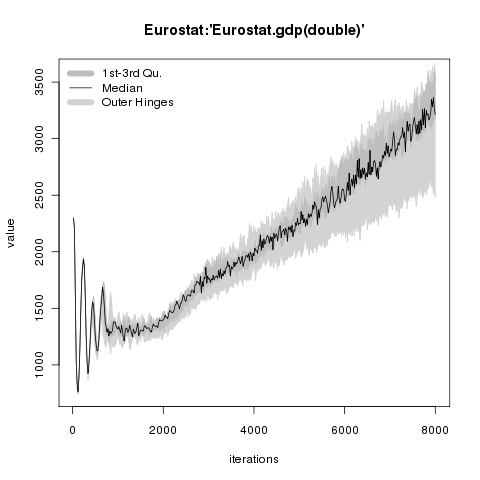
\includegraphics[width=8cm]{./transient/tax_0.08/Eurostat-gdp.png}
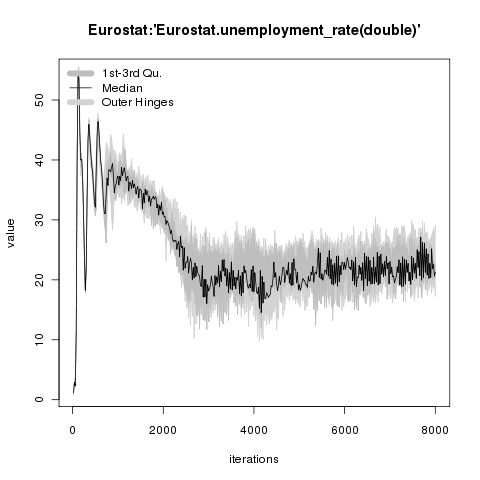
\includegraphics[width=8cm]{./transient/tax_0.08/Eurostat-unemployment_rate.png}\\
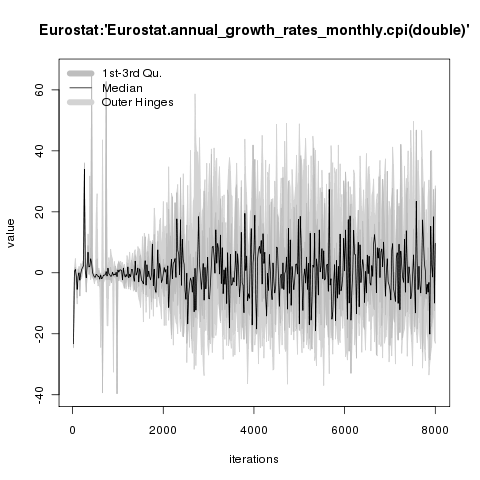
\includegraphics[width=8cm]{./transient/tax_0.08/Eurostat-cpi.png}
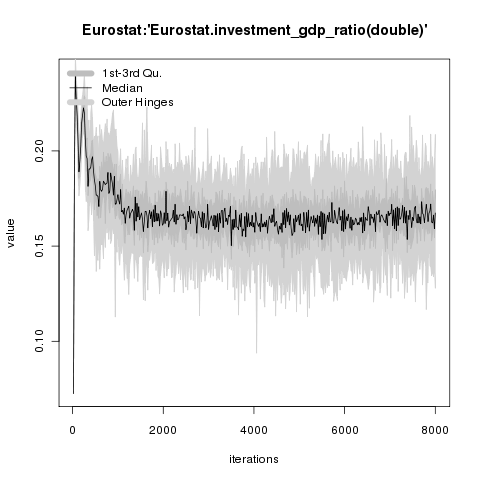
\includegraphics[width=8cm]{./transient/tax_0.08/Eurostat-investment_gdp_ratio.png}
\end{minipage}
\caption{Time series plots for 20 batch runs. GDP, unemployment rate, inflation rate and investment/GDP ratio.}
\label{Figure: transient time}
\end{figure}

%\subsubsection*{Distribution across batch runs}

\begin{figure}[ht!]
\centering\leavevmode
\begin{minipage}{17cm}
\centering\leavevmode
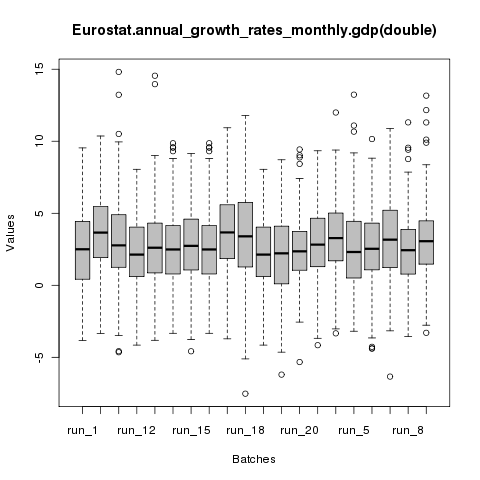
\includegraphics[width=8cm]{./benchmark_plots/Eurostat-annual_growth_rates_monthly-gdp-batches.png}
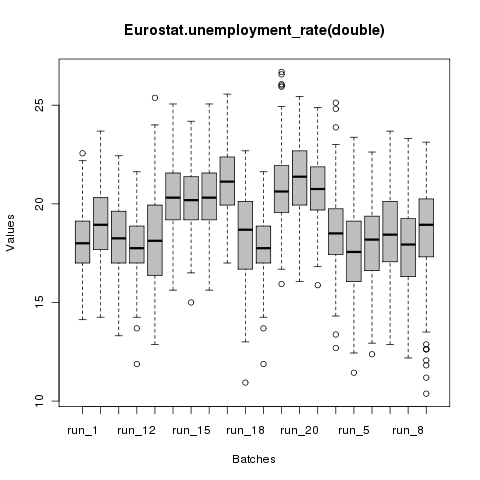
\includegraphics[width=8cm]{./benchmark_plots/Eurostat-unemployment_rate-batches.png}\\
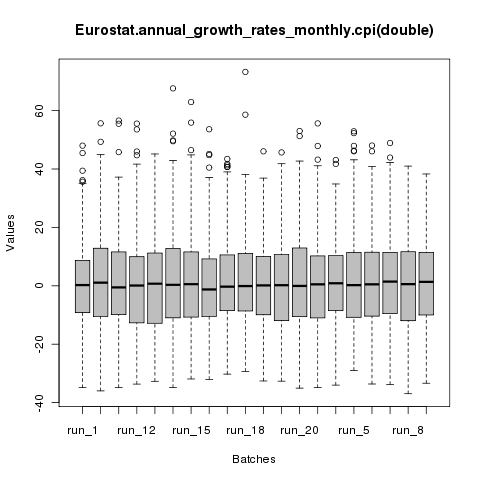
\includegraphics[width=8cm]{./benchmark_plots/Eurostat-cpi-batches.png}
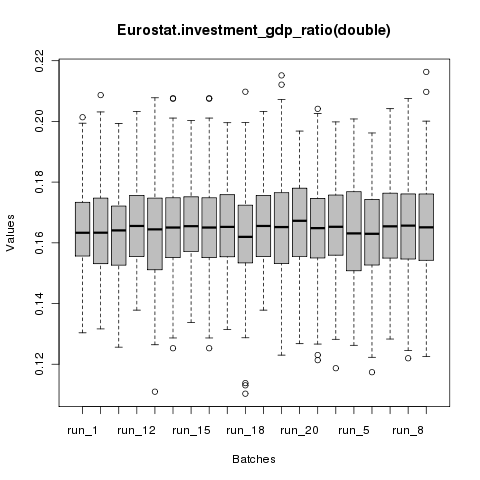
\includegraphics[width=8cm]{./benchmark_plots/Eurostat-investment_gdp_ratio-batches.png}
\end{minipage}
\caption{Box plots for separate runs of GDP, unemployment rate, inflation rate and investment/GDP ratio.}
\label{Figure: run batch}
\end{figure}

\begin{comment}
\documentclass{article}
\usepackage{epsfig,graphicx,verbatim, boxedminipage, url}
\begin{document}
\end{comment}

\begin{comment}
%\subsubsection*{Eurostat macrodata}
\begin{figure}[H!]
\centering\leavevmode
\begin{minipage}{14cm}
\centering\leavevmode
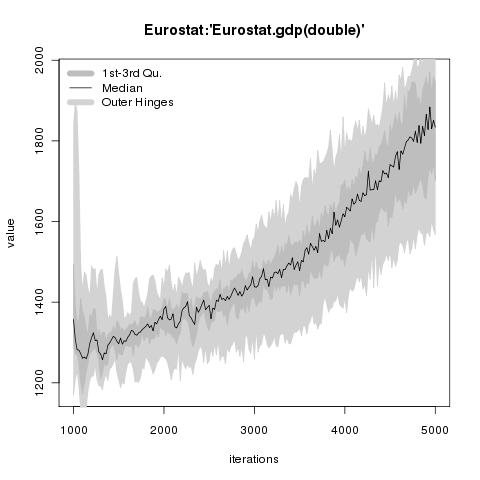
\includegraphics[width=6cm]{./png/tax_0.10/Eurostat-gdp.png}
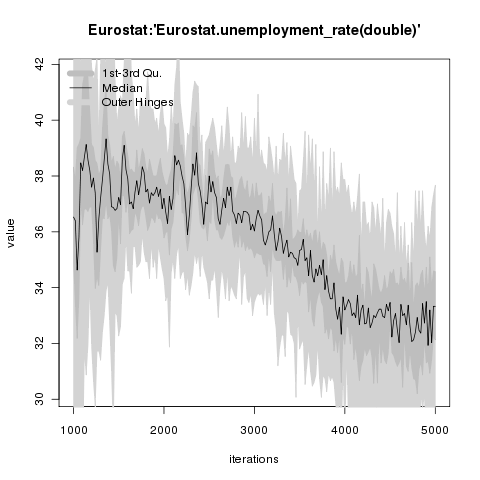
\includegraphics[width=6cm]{./png/tax_0.10/Eurostat-unemployment_rate.png}
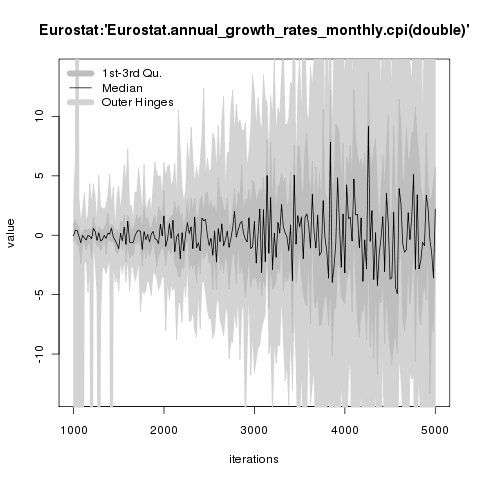
\includegraphics[width=6cm]{./png/tax_0.10/Eurostat-annual_growth_rates_monthly_cpi.png}
\end{minipage}
\caption{Eurostat: GDP, unemployment rate and inflation rate (annual, measured monthly).}
\label{Figure: Eurostat macrodata}
\end{figure}
\end{comment}

%\begin{comment}
%\subsubsection*{Growth rates}
\begin{figure}[H!]
\centering\leavevmode
\begin{minipage}{14cm}
\centering\leavevmode
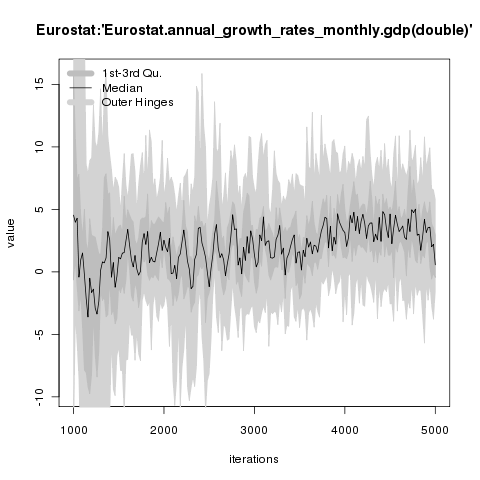
\includegraphics[width=6cm]{./png/tax_0.10/Eurostat-annual_growth_rates_monthly_gdp.png}
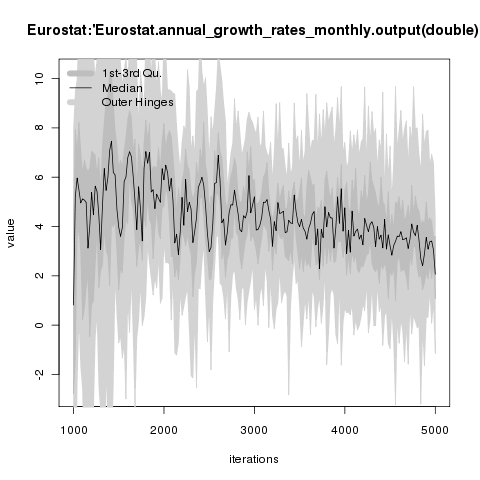
\includegraphics[width=6cm]{./png/tax_0.10/Eurostat-annual_growth_rates_monthly_output.png}\\
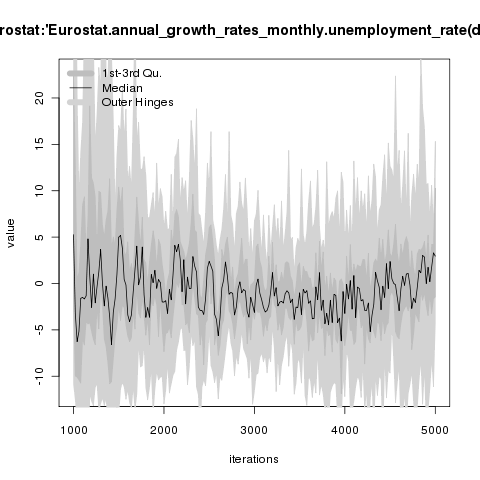
\includegraphics[width=6cm]{./png/tax_0.10/Eurostat-annual_growth_rates_monthly_unemployment_rate.png}
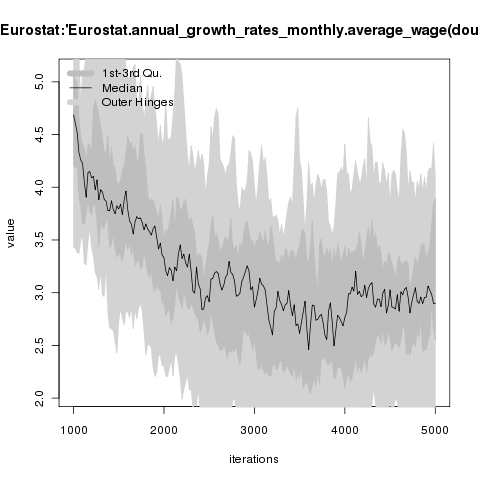
\includegraphics[width=6cm]{./png/tax_0.10/Eurostat-annual_growth_rates_monthly_average_wage.png}
\end{minipage}
\caption{Annual growth rates (with respect to same month in the previous year): GDP, output, unemployment rate and avgerage wage. Tax: $10\%$.}
\label{Figure: Eurostat macrodata growth rates}
\end{figure}
\clearpage
%\end{comment}

%\pagebreak
%\subsubsection*{Government}
\begin{figure}[H!]
\centering\leavevmode
\begin{minipage}{14cm}
\centering\leavevmode
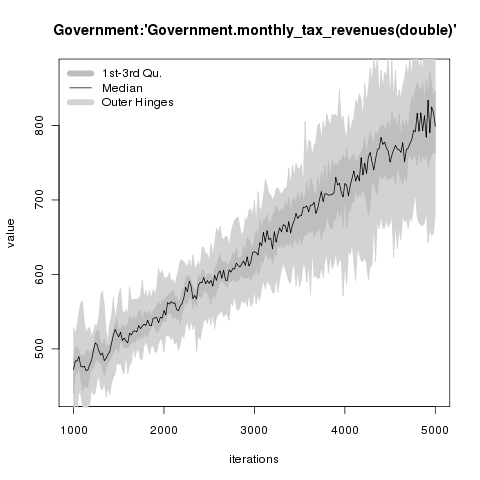
\includegraphics[width=6cm]{./png/tax_0.10/Government-monthly_tax_revenues.png}
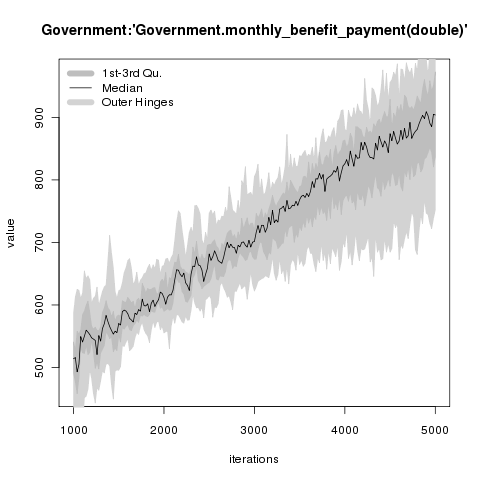
\includegraphics[width=6cm]{./png/tax_0.10/Government-monthly_benefit_payment.png}\\
%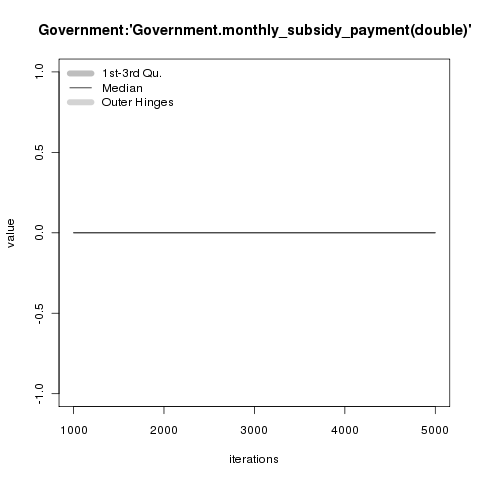
\includegraphics[width=6cm]{./png/tax_0.10/Government-monthly_subsidy_payment.png}
%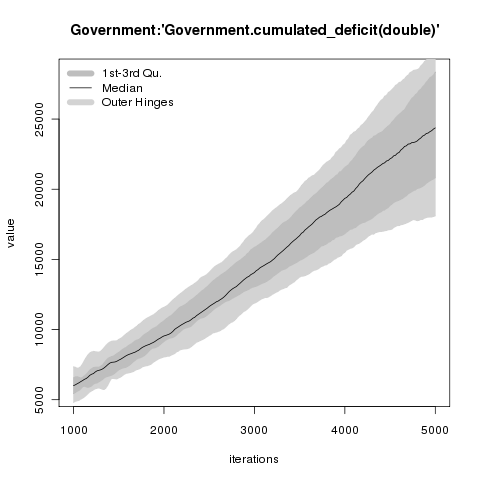
\includegraphics[width=6cm]{./png/tax_0.10/Government-cumulated_deficit.png}
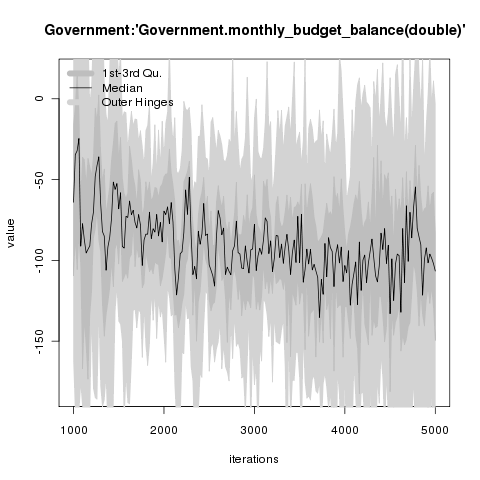
\includegraphics[width=6cm]{./png/tax_0.10/Government-monthly_budget_balance.png}
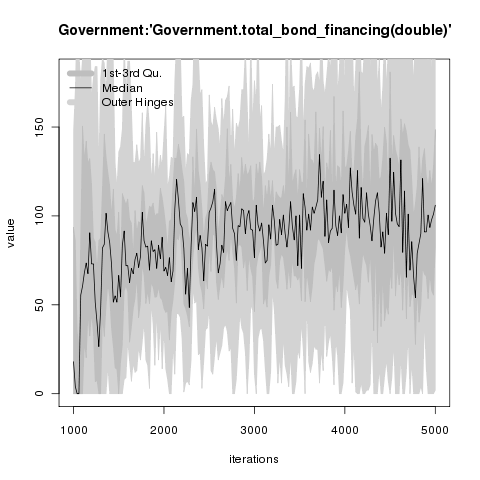
\includegraphics[width=6cm]{./png/tax_0.10/Government-total_bond_financing.png}
%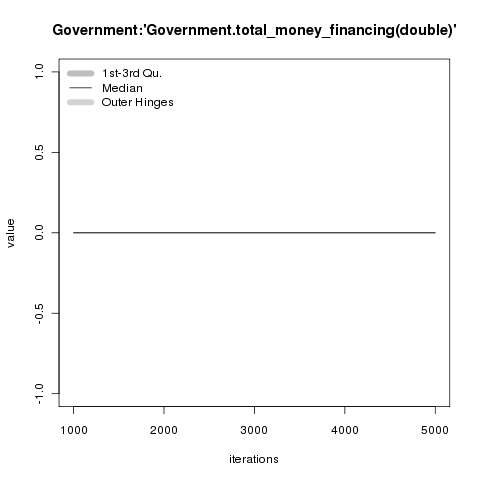
\includegraphics[width=6cm]{./png/tax_0.10/Government-total_money_financing.png}
\end{minipage}
\caption{Government finances.}
\label{Figure: Government}
\end{figure}
\clearpage

%\pagebreak
%\subsubsection*{Firms}
\begin{figure}[H!]
\centering\leavevmode
\begin{minipage}{14cm}
\centering\leavevmode
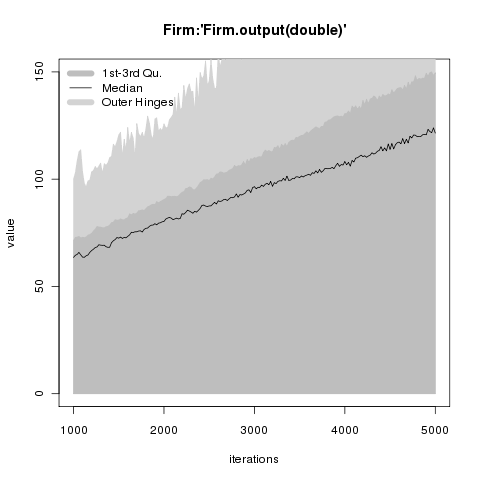
\includegraphics[width=6cm]{./png/tax_0.10/Firm-output.png}
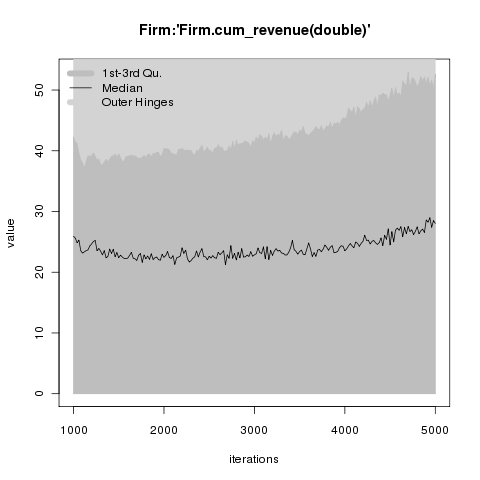
\includegraphics[width=6cm]{./png/tax_0.10/Firm-cum_revenue.png}\\
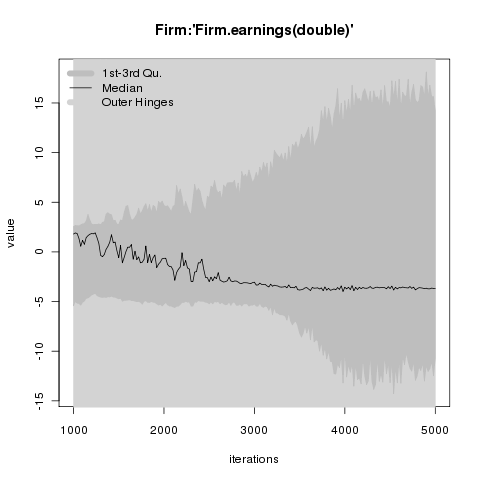
\includegraphics[width=6cm]{./png/tax_0.10/Firm-earnings.png}
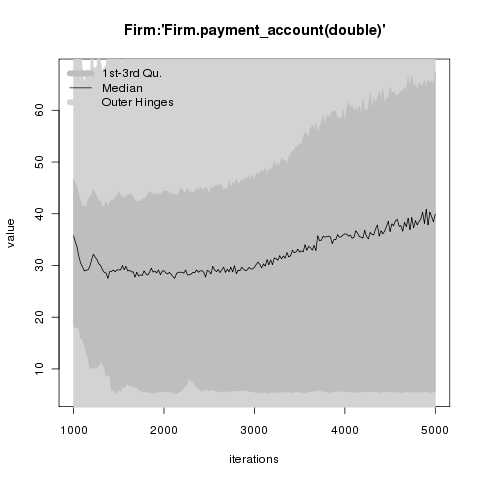
\includegraphics[width=6cm]{./png/tax_0.10/Firm-payment_account.png}\\
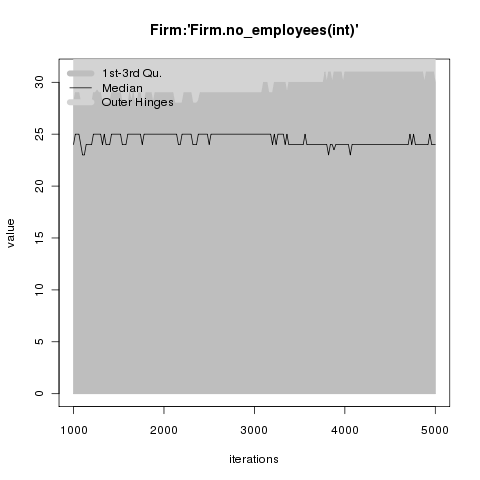
\includegraphics[width=6cm]{./png/tax_0.10/Firm-no_employees.png}
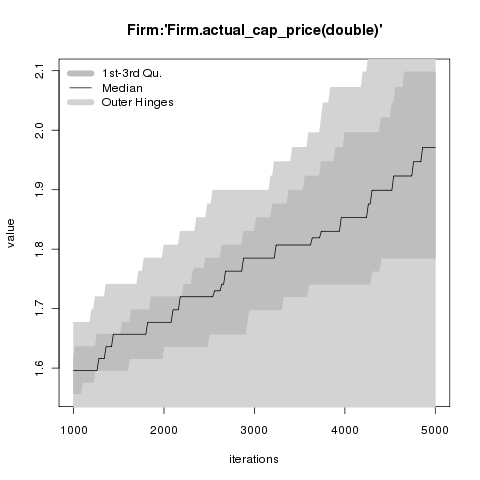
\includegraphics[width=6cm]{./png/tax_0.10/Firm-actual_cap_price.png}
%\includegraphics[width=6cm]{./png/tax_0.10/Firm-bankruptcy_state.png}
\end{minipage}
\caption{Firm production data.}
\label{Figure: Firm Production}
\end{figure}

\begin{figure}[H!]
\centering\leavevmode
\begin{minipage}{14cm}
\centering\leavevmode
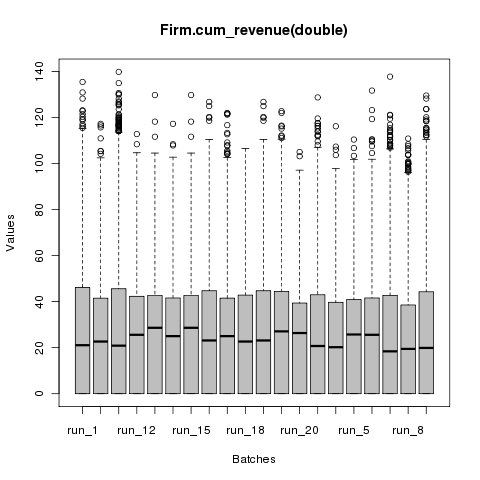
\includegraphics[width=6cm]{./png/tax_0.10/Firm-cum_revenue-batches.png}
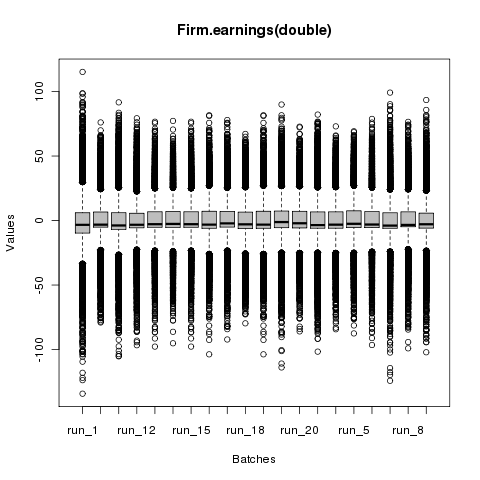
\includegraphics[width=6cm]{./png/tax_0.10/Firm-earnings-batches.png}
\end{minipage}
\caption{Firm production data, all batch runs.}
\label{Figure: Firm Production batch}
\end{figure}
\clearpage


%\subsubsection*{Financial Data}
\begin{figure}[H!]
\centering\leavevmode
\begin{minipage}{14cm}
\centering\leavevmode
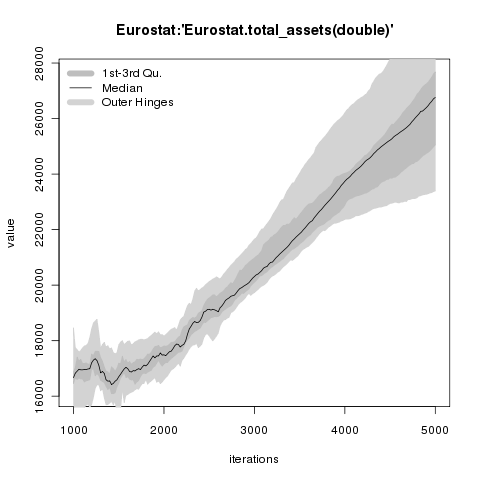
\includegraphics[width=6cm]{./png/tax_0.10/Eurostat-total_assets.png}
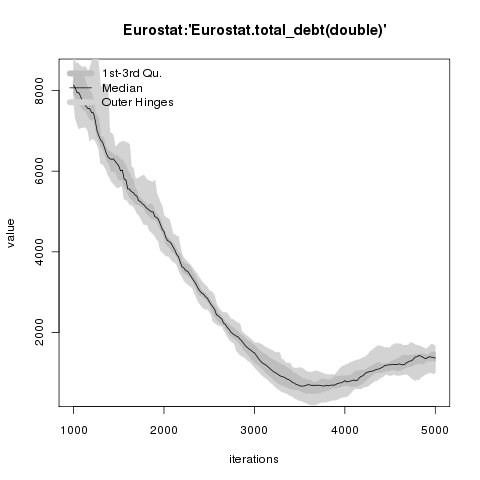
\includegraphics[width=6cm]{./png/tax_0.10/Eurostat-total_debt.png}\\
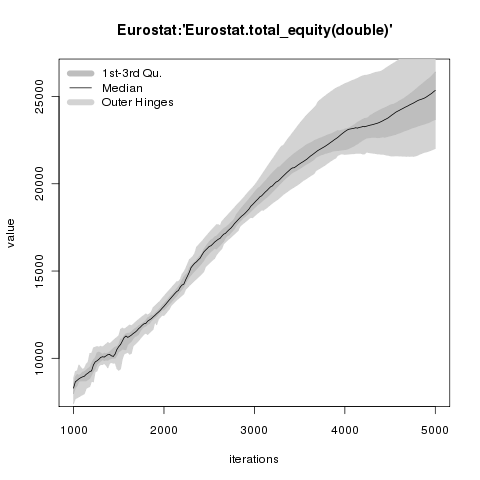
\includegraphics[width=6cm]{./png/tax_0.10/Eurostat-total_equity.png}
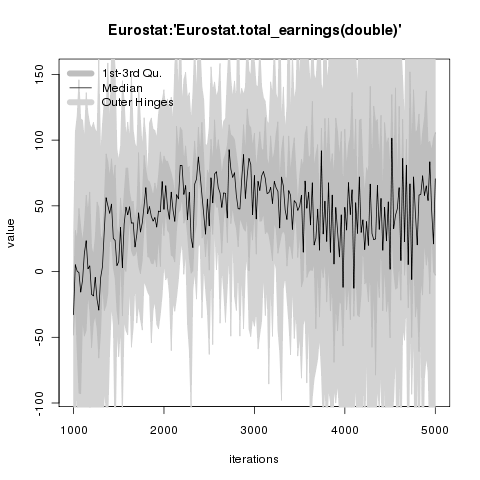
\includegraphics[width=6cm]{./png/tax_0.10/Eurostat-total_earnings.png}\\
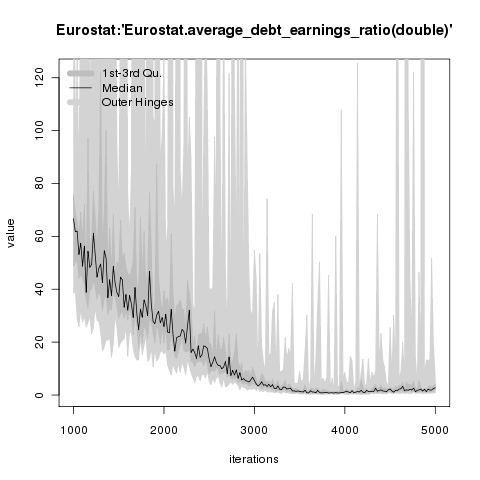
\includegraphics[width=6cm]{./png/tax_0.10/Eurostat-average_debt_earnings_ratio.png}
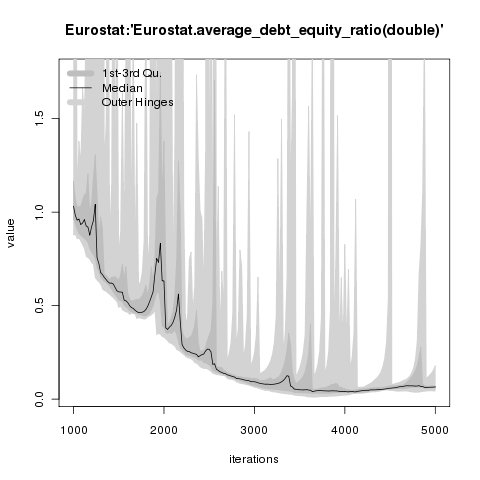
\includegraphics[width=6cm]{./png/tax_0.10/Eurostat-average_debt_equity_ratio.png}
\end{minipage}
\caption{Firm financial data.}
\label{Figure: Firm Financial Data}
\end{figure}


%\pagebreak
%\subsubsection*{Labour Market}
\begin{figure}[H!]
\centering\leavevmode
\begin{minipage}{14cm}
\centering\leavevmode
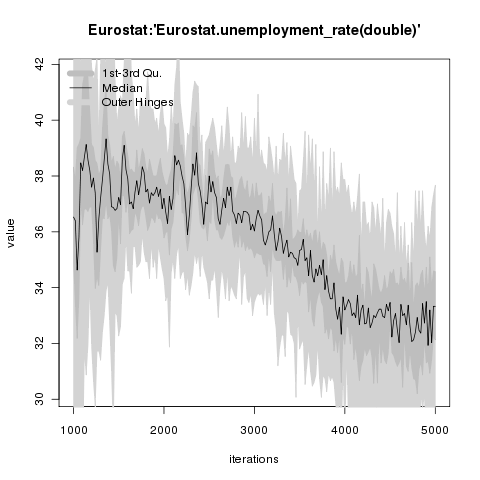
\includegraphics[width=6cm]{./png/tax_0.10/Eurostat-unemployment_rate.png}
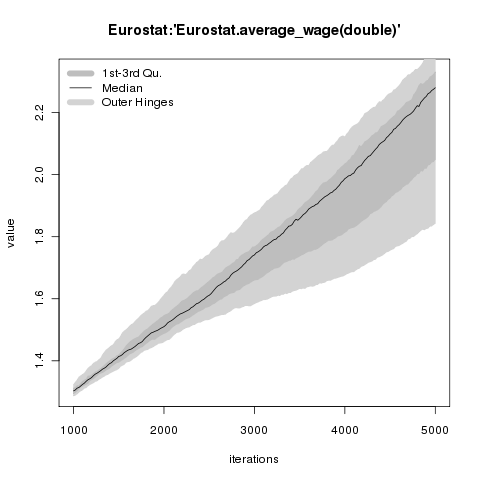
\includegraphics[width=6cm]{./png/tax_0.10/Eurostat-average_wage.png}\\
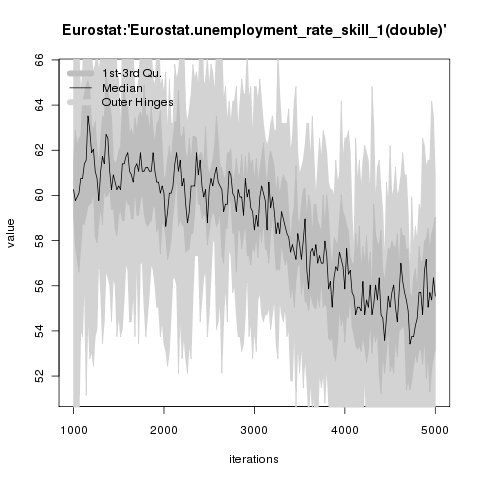
\includegraphics[width=6cm]{./png/tax_0.10/Eurostat-unemployment_rate_skill_1.png}
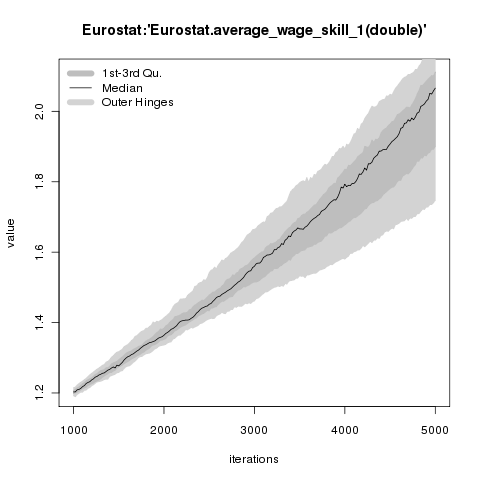
\includegraphics[width=6cm]{./png/tax_0.10/Eurostat-average_wage_skill_1.png}\\
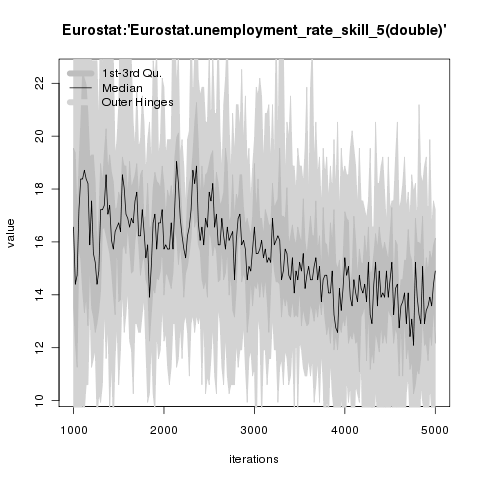
\includegraphics[width=6cm]{./png/tax_0.10/Eurostat-unemployment_rate_skill_5.png}
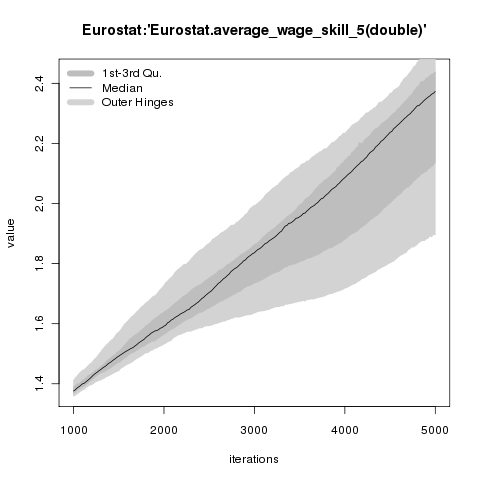
\includegraphics[width=6cm]{./png/tax_0.10/Eurostat-average_wage_skill_5.png}
\end{minipage}
\caption{Labour market data.}
\label{Figure: Labour Market}
\end{figure}


\begin{figure}[H!]
\centering\leavevmode
\begin{minipage}{14cm}
\centering\leavevmode
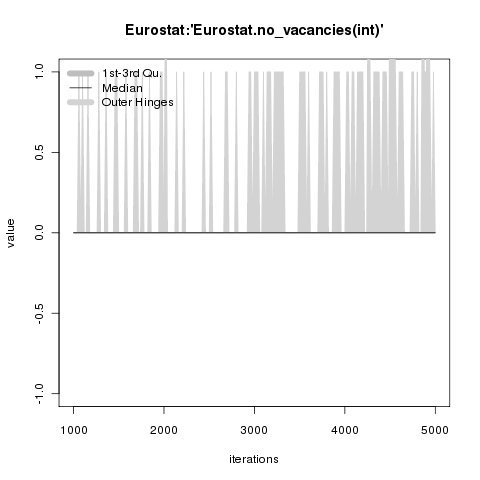
\includegraphics[width=6cm]{./png/tax_0.10/Eurostat-no_vacancies.png}
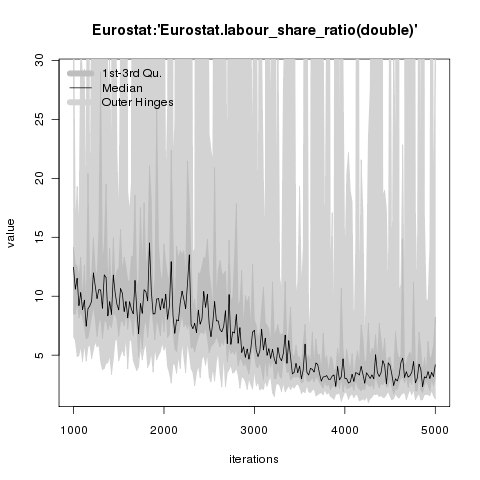
\includegraphics[width=6cm]{./png/tax_0.10/Eurostat-labour_share_ratio.png}\\
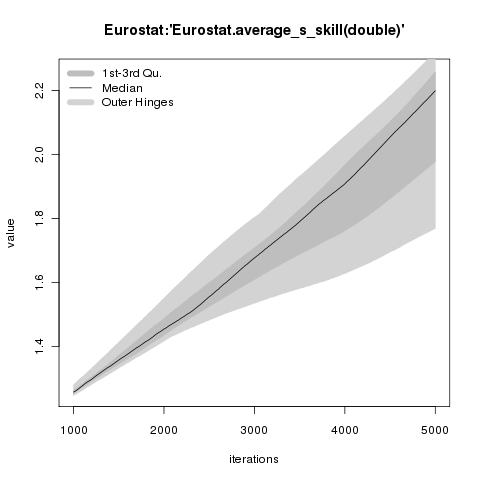
\includegraphics[width=6cm]{./png/tax_0.10/Eurostat-average_s_skill.png}
\end{minipage}
\caption{Labour market data (cont).}
\label{Figure: Labour Market 2}
\end{figure}

\clearpage


%\subsubsection*{Consumption Market}
\begin{figure}[H!]
\centering\leavevmode
\begin{minipage}{14cm}
\centering\leavevmode
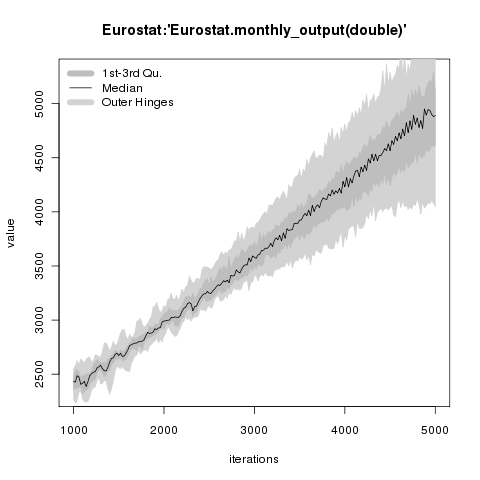
\includegraphics[width=6cm]{./png/tax_0.10/Eurostat-monthly_output.png}
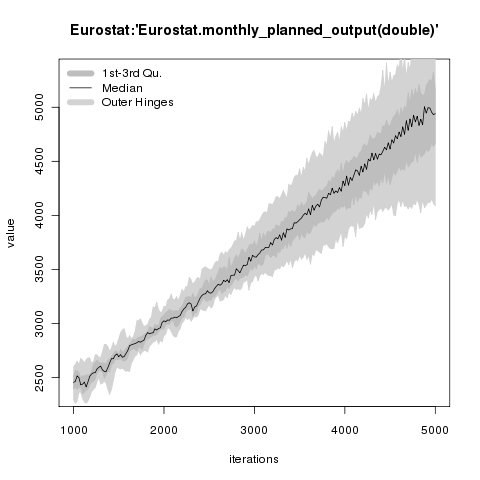
\includegraphics[width=6cm]{./png/tax_0.10/Eurostat-monthly_planned_output.png}\\
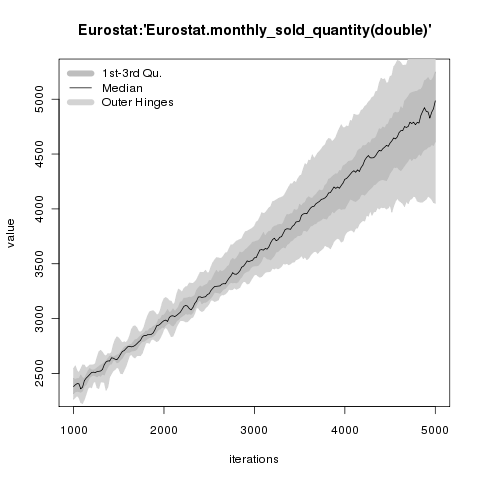
\includegraphics[width=6cm]{./png/tax_0.10/Eurostat-monthly_sold_quantity.png}
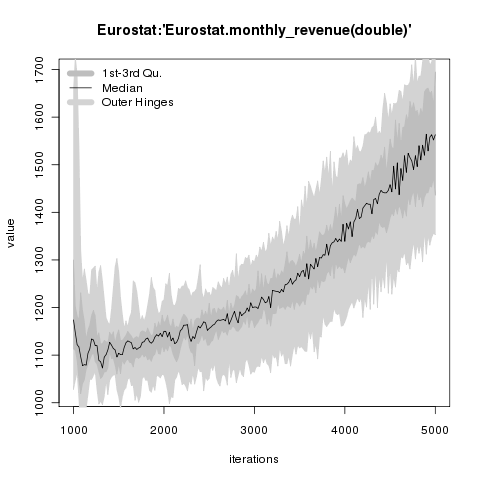
\includegraphics[width=6cm]{./png/tax_0.10/Eurostat-monthly_revenue.png}\\
\includegraphics[width=6cm]{./png/tax_0.10/Eurostat-firm_average_productivity.png}
\includegraphics[width=6cm]{./png/tax_0.10/Eurostat-firm_average_productivity_progress.png}
\end{minipage}
\caption{Consumption goods market.}
\label{Figure: Consumption Market}
\end{figure}
\clearpage


%\pagebreak
%\subsubsection*{Credit market}
\begin{figure}[H!]
\centering\leavevmode
\begin{minipage}{14cm}
\centering\leavevmode
\includegraphics[width=6cm]{./png/tax_0.10/Bank-cash.png}
\includegraphics[width=6cm]{./png/tax_0.10/Bank-deposits.png}\\
\includegraphics[width=6cm]{./png/tax_0.10/Bank-total_credit.png}
\includegraphics[width=6cm]{./png/tax_0.10/Bank-equity.png}\\
\includegraphics[width=6cm]{./png/tax_0.10/Bank-ecb_debt.png}
\includegraphics[width=6cm]{./png/tax_0.10/Bank-total_dividends.png}
\end{minipage}
\caption{Credit market data.}
\label{Figure: Credit Market}
\end{figure}
%\clearpage

%\end{document}

\begin{figure}[ht!]
\centering\leavevmode
\begin{minipage}{7.5cm}
\centering\leavevmode
\includegraphics[width=6cm]{./batch/Eurostat-annual_growth_rates_monthly-gdp-scenarios.png}\\
\includegraphics[width=6cm]{./batch/Eurostat-unemployment_rate-scenarios.png}\\
\includegraphics[width=6cm]{./batch/Eurostat-investment_gdp_ratio-scenarios.png}
\end{minipage}
\caption{Parameter sensitivity analysis for different tax rates of $0-8\%$ and $10,15,20\%$. Results are for $20$ batch runs over $4000$ periods (using periods $4001$ to $8000$).}
\label{Figure: scenarios}
\end{figure}


